\documentclass[12pt]{article}
\usepackage{a4wide}
\usepackage{latexsym}
\usepackage{amssymb}
\usepackage{epic}
\usepackage{graphicx}
\usepackage[shortlabels]{enumitem}
\usepackage{amsmath}
%\pagestyle{empty}
\newcommand{\tr}{\mbox{\sf true}}
\newcommand{\fa}{\mbox{\sf false}}
\newcommand{\bimp}{\leftrightarrow}


\begin{document}

\section*{Automated Reasoning - Assignment series 1 }

\begin{center}
P.T. Jager, BSc. \\
Radboud universiteit Nijmegen\\
email: {\tt p.jager@student.ru.nl}
\end{center}

\subsection*{Problem 1: Magic factory}

Six trucks have to deliver various obscure building blocks to a special 
factory. There are five types of building blocks:
\begin{enumerate}[(a)]
	\item Nuzzles - 4 pallets - 700 kg 
	\item Skipples - 8 pallets - 1000 kg - \textit{Need to be cooled in
		one of the two cooled trucks}
	\item Crottles - 10 pallets - 1500 kg - \textit{Can not be in the same truck
		as Prittles}
	\item Dupples - 5 pallets - 100 kg - \textit{Not more than 2 pallets per
		truck}
	\item Prittles - $\geq 1$ pallets - 800 kg - \textit{Can not be in same 
		truck as Crottles}
\end{enumerate}
All trucks can cary a maximum of 8 pallets or 7800 kg (whichever is reached 
first.)
What is the maximum number of Prittles that can be delivered and how would the
pallets be divided over the 6 trucks?

For a complete description of the problem please see assignment. 

\subsubsection*{Solution:}

We generalize the solution for any $a$ Nuzzles, $b$ Skipples, $c$ Crottles, 
$d$ Dupples, $e$ Prittles and $f$ trucks.

For doing so we introduce $f*a + f*b + f*c + f*d + f*e$ variables which 
represent each possible pallet in each possible truck: 
\begin{enumerate}[(a)]
	\item $nuzzle_{tn}$ for $t=1,\ldots,f$ and $n=1,\ldots,a$
	\item $skipple_{tn}$ for $t=1,\ldots,f$ and $n=1,\ldots,b$
	\item $crottle_{tn}$ for $t=1,\ldots,f$ and $n=1,\ldots,c$
	\item $dupple_{tn}$ for $t=1,\ldots,f$ and $n=1,\ldots,d$
	\item $prittle_{tn}$ for $t=1,\ldots,f$ and $n=1,\ldots,e$
\end{enumerate}
All of these variables are either $0$ or $1$, when the $nuzzle_{tn}$ 
is $1$ for some $t,n$ then nuzzle $n$ is in truck $t$. Similar for the other 
building blocks.

\vspace{3mm}

In the following formulas we will use $blocks$ as a shorthand for ${nuzzle, 
skipple, crottle, dupple, prittle}$ and use $p_{tn}$ with $p \in blocks$
as a shorthand notation for eg. $nuzzle_{tn}$. The function $num(p)$ is assumed 
to give the number of desired pallets to move of a certain block $p$, eg.
$num(dupple) = d$. Similar, the function $weight(p)$ gives the weight of a 
certain pallet $p$.

\vspace{3mm}

For each building block the correct \emph{amount} of blocks need to be
transported. This is expressed in formula
\begin{equation} \label{eq:amount}
  \bigwedge_p^{blocks} (\sum_{t=1}^{f} \sum_{n=1}^{num(p)} p_{tn} = num(p))
\end{equation}

The combined \emph{weight} of all pallets in an truck can not exceed 7800kg. 
This is expressed in the formula
\begin{equation} \label{eq:weight}
 \bigwedge_t^f (\sum_p^{blocks} \sum_n^{num(p)} weight(p_{tn}) \leq 7800)
\end{equation}

Because all pallets have $f$ different positions they could be in (one for each
truck), it is necessary to express that each \emph{distinct} pallet (numbered 
$n$) is in exactly one truck.
\begin{equation} \label{eq:distinct}
  \bigwedge_p^{blocks} \bigwedge_n^{num(p)} (\sum_{t=1}^f p_{tn} = 1)
\end{equation}

The problem states that \emph{no 2 duples} can be in any truck. 
That is, for each truck the number of duples should be $\leq 1$. 
\begin{equation} \label{eq:valuable}
  \bigwedge_{t=1}^f (\sum_{n=1}^d dupple_{tn} \leq 1)
\end{equation}

All Skipples should be in one of two \emph{cooled} trucks. We give these trucks
numbers 1 and 2. 
\begin{equation} \label{eq:cooled}
  \sum_{t=1}^2 \sum_{n=1}^b p_{tn} = b
\end{equation}

All trucks should \emph{not contain Prittles if they contain Crottles}. That is,
if the number of Crottles in a truck is $\geq 1$ then the number of Prittles 
should be 0. If this
property holds then the reverse is also true (since containment is commutative).
When expressing this formula we use the function \emph{ite} (if-then-else) which
evaluates to its second argument when the first one evaluates to $true$ and 
evaluates to its third argument otherwise.
\begin{equation} \label{eq:explosive}
  \bigwedge_t^f ite 	(\sum_{n=1}^c crottle_{tn} \geq 1)\  
						(\sum_{n=1}^e prittle_{tn} = 0)\ 
						true 
\end{equation}

One additional needed constraint has to with the choice to represent $p_{tn}$
as a number. This constraint states that all $p_{tn}$ are either 1 or 0, that is
truck $t$ contains pallet $p$ numbered $n$ (1) or not (0).
\begin{equation} \label{eq:range}
  \bigwedge_p^{blocks} \bigwedge_{t=1}^f \bigwedge_{n=1}^{num(p)} 
	p_{tn} = 0 \vee p_{tn} = 1
\end{equation}

The total formula consists of the conjunction of all these formulas.

This formula is easily expressed in YICES syntax.

To now find what the maximum number of Prittles is we vary the number $e$. 
Through these experiments it is found that 18 is the largest number of Prittles
that can be transported within the given constraints.
Applying {\tt yices assignment1.ys} with $e=18$ yields a result almost 
instantly:

{\footnotesize

{\tt sat }

{\tt (= stipple6\_3 0)}

{\tt (= dupple4\_2 0)}

{\tt (= stipple3\_4 0)}

{\tt (= stipple4\_4 0)}

{\tt (= dupple6\_2 0)}

{\tt (= stipple1\_6 1)}

{\tt (= dupple5\_1 1)}

{\tt (= prittle6\_15 0)}

$\cdots \cdots$ }.

The following table expresses which packet is in which truck

\vspace{3mm}

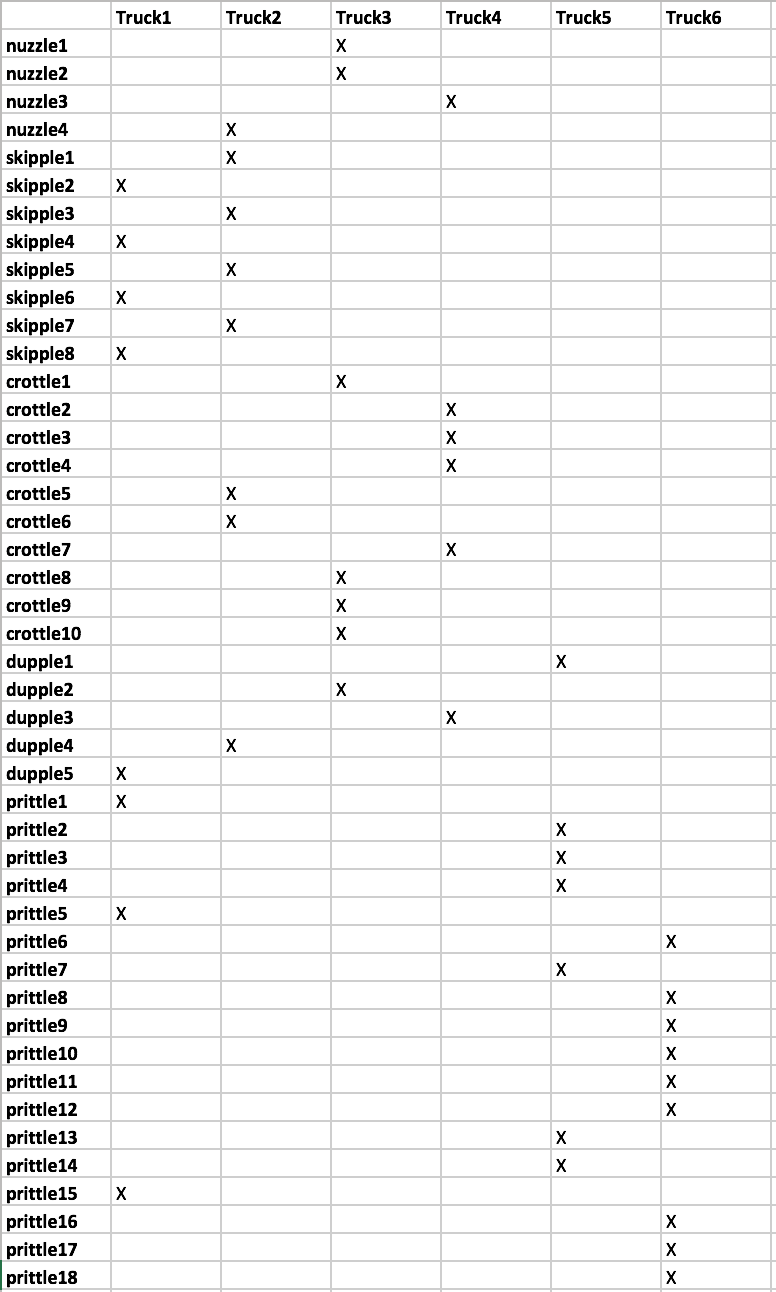
\includegraphics[angle=0]{one.png}

\subsection{Problem 2: Chip design}

Give a chip design containing eight regular and three power components 
satisfying the following constraints:
\begin{itemize}
	\item The width of the chip is 29 and the height is 22.
	\item All power components have width 4 and height 2.
	\item The sizes of the eight regular components are $9*7$,
		$12*6,$ $10*7,$ $18*5,$ $20*4,$
		$10*6,$ $8*6$ and $10*8$ respectively.
	\item All components may be turned 90, but may not overlap.
	\item In order to get power, all regular components should directly be
		connected to a power component, that is, an edge of the
		component should have at least one point in common with an edge
		of the power component.
	\item Due to limits on heat production the power components should be
		not too close: their centres should differ at least $17$ in
		either the $x$ direction or the $y$ direction (or both).
\end{itemize}

\subsubsection{Solution}
We define the set $PC$ of all power components, the set $RC$ of all regular
components and the set $C = PC \cup RC$. Furthermore for every $c \in C$ we
define $x_c, y_c$ for the x and y coordinate of its bottom left corner and
$h_c, w_c$ for its width and height. 

\vspace{3mm}

The following formulas express the above constraints:

\vspace{3mm}

All components should fit within the board, therefore:
\begin{equation} 
	\forall c \in C : (0 \leq x_c \le (29-w_c)) \wedge 
		(0 \leq y_c \le (22-h_c))
\end{equation}

\vspace{3mm}

Components should not overlap, therefore they should either be completely
left, right, above or below every other component. 
\begin{equation}
	\forall c \in C : \forall c' \in C \setminus \{c\} :
		(x_{c'} \geq x_c + w_c) \vee
		(x_{c'} + w_{c'} \le x_c) \vee
		(y_{c'} \geq y_c + h_c) \vee
		(y_{c'} + h_{c'} \le y_c)
\end{equation}

\vspace{3mm}

Each regular component should share an edge with at least on power component.
\begin{multline}
	\forall r \in RC : \exists p \in PC :
		(x_p \leq x_r \le x_p+h_p \wedge (y_r=y_p+h_p \vee y_r+h_r=y_p)  \\  
		\vee (x_p \leq x_r \le x_p+w_p \wedge (x_r=x_p+w_p \vee x_r+w_r=x_p)
\end{multline}

\vspace{3mm}

Power components should differ at least 17 in the position of their centers.
\begin{multline}
	\forall r \in RC : \forall r' \in RC \setminus \{r\} :
		|(x_r + w_r/2) - (x_{r'} + w_{r'}/2)| \geq 17 \\  
		\vee |(y_r + h_r/2) - (y_{r'} + h_{r'}/2)| \geq 17
\end{multline}

Each component can be rotated 90$^{\circ}$. We assume the function 
$width(c)$ for the width and $height(c)$ for the hight of a component $c$ as
specified in the constraints. 
\begin{multline}
	\forall c \in C : (w_c = width(c) \wedge h_c = height(c))
		\vee (w_c = height(c) \wedge h_c = width(c))
\end{multline}

The complete formula consists of the conjunction of these formulas. This
formula is easily expressed in YICES syntax. If we replace all universal
quantifiers by conjunctions:
\begin{equation}
	\forall c \in C \rightarrow \bigwedge_c^C
\end{equation}
and all existential quantifiers by disjunctions:
\begin{equation}
	\exists c \in C \rightarrow \bigvee_c^C
\end{equation}
it can even be expressed without any quantification, this makes YICES more
reliable in providing a correct result.

This yields: ARGH UNSAT, HOEZO IS DIT UNSAT $:/$

\end{document}
